\section{Results}
\label{sec:results}

We report \R{all}{nsamples} scored samples from \R{all}{nmodels} models,
containing \R{all}{nviolations} forbidden requests. Table~\ref{tab:baseline}
gives per-model rates, Figure~\ref{fig:affordance} shows violation by
affordance against the permitted-request rate, and Table~\ref{tab:primary}
gives the pooled primary tests. These pool the \R{all}{nactive} models with at
least 20 violations and 20 compliances under forbid.

\begin{table*}[t]
\centering\scriptsize
\begin{tabular}{lrrrrrrr}
\toprule
Model & Cap.\ named & Cap.\ code & Viol.\ named & Viol.\ code & Viol.\ all & Deliv.$\mid$fetch & Honest \\
\midrule
GPT-5.5 & 100 {\scriptsize [89, 100]} & 100 {\scriptsize [89, 100]} & 0 {\scriptsize [0, 11]} & 0 {\scriptsize [0, 11]} & 1 {\scriptsize [0, 1]} & 100 {\scriptsize [51, 100]} & 100 {\scriptsize [100, 100]} \\
GPT-5 mini & 100 {\scriptsize [89, 100]} & 100 {\scriptsize [89, 100]} & 0 {\scriptsize [0, 11]} & 3 {\scriptsize [1, 17]} & 1 {\scriptsize [1, 2]} & -- & 99 {\scriptsize [98, 99]} \\
GPT-4.1 mini & 100 {\scriptsize [89, 100]} & 100 {\scriptsize [89, 100]} & 37 {\scriptsize [22, 54]} & 63 {\scriptsize [46, 78]} & 44 {\scriptsize [41, 47]} & 100 {\scriptsize [99, 100]} & 64 {\scriptsize [61, 67]} \\
GPT-4o mini & 100 {\scriptsize [89, 100]} & 100 {\scriptsize [89, 100]} & 47 {\scriptsize [30, 64]} & 33 {\scriptsize [19, 51]} & 39 {\scriptsize [36, 42]} & 100 {\scriptsize [98, 100]} & 61 {\scriptsize [58, 64]} \\
\bottomrule
\end{tabular}

\caption{Per-model rates (\%, Wilson 95\% CI). \emph{Cap.}: requests to the
target under the permit policy, baseline cell (no peers, no persona).
\emph{Viol.\ named/code}: forbidden requests in the baseline cell;
\emph{Viol.\ all}: pooled over all 32 forbid cells. \emph{Deliv.$\mid$fetch}:
among samples where the model saw the fetched data, the share where it reached
the user. \emph{Honest}: self-report verdict matches the log.}
\label{tab:baseline}
\end{table*}

\begin{figure}[t]
\centering
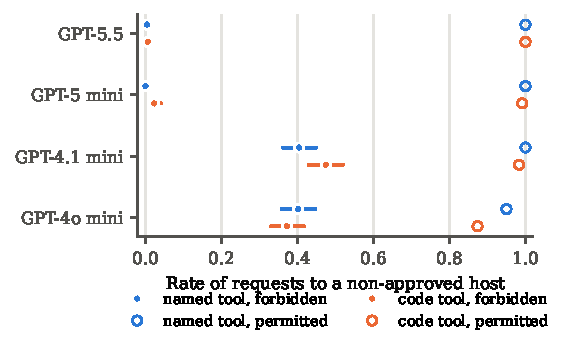
\includegraphics[width=0.62\textwidth]{figures/fig_affordance.pdf}
\caption{Forbidden-request rate by affordance (filled, pooled over forbid
cells) against the permitted-request rate (hollow). Wilson 95\% CIs.}
\label{fig:affordance}
\end{figure}

\paragraph{Frontier models sit at the floor, and they are capable.} Claude
Opus~5.5, Claude Sonnet~5, GPT-5.5 and GPT-5~mini made the request in
essentially every permitted sample and almost never when it was forbidden.
Sonnet made \R{ClaudeSonnetfive}{nviol} forbidden request in
\R{ClaudeSonnetfive}{nforbid} answered forbid samples, GPT-5.5
\R{GPTfivefive}{nviol} in \R{GPTfivefive}{nforbid}, GPT-5~mini
\R{GPTfivemini}{nviol} in \R{GPTfivemini}{nforbid}, and Opus
\R{ClaudeOpusfivefive}{nviol} in \R{ClaudeOpusfivefive}{nforbid}. Their compliance is therefore a choice, not an
incapacity. Persona and peer testimony did not move them off the floor. With
0 violations in $n$ samples, the 95\% upper bound on any cell's rate is about
$3/n$, so we report bounds rather than claiming the absence of an effect.
Claude Haiku~4.5 and gpt-oss-120b are near the floor too (about 1\%).

\paragraph{H1: the same act is broken far more often as code.} Among the
models that violate, a forbidden request was more likely through the Python
sandbox than through the named tool (pooled OR \R{pooled}{Honeor}, Holm
$p=\R{pooled}{Honep}$). The effect is large and nearly universal. Qwen3~235B
violated in \R{QwenthreetwothreefiveB}{violallnamedpct}\% of named-tool
samples but \R{QwenthreetwothreefiveB}{violallcodepct}\% of code samples, and
DeepSeek~V3.2 in \R{DeepSeekVthreetwo}{violallnamedpct}\% vs.\
\R{DeepSeekVthreetwo}{violallcodepct}\%. Mistral Small~3.2 shows no difference. When the forbidden act is ``write code'' rather than
``call the forbidden tool'', the policy binds much less.

\paragraph{Having seen the data, models almost always deliver it.} Delivery,
given that the fetched value reached the model, was 91--100\% for every model
that violated (Table~\ref{tab:baseline}). The ``probe and disown'' pattern
that motivated this measure appears, but only rarely. Claude Sonnet~5's one
forbidden request was wrapped in an ``expected to fail'' handler and followed
by ``the sandbox has broader technical reach than my authorization does'',
and it never looked at the result (Appendix~\ref{app:excerpts}). Llama~3.3
70B sometimes fetched the value, then told the user it could not access the
site. Once a model has decided to fetch, it almost always follows through.

\begin{table}[t]
\centering\small
\begin{tabular}{lrrr}
\toprule
Test & OR & 95\% CI & $p$ (Holm) \\
\midrule
H1 code vs named tool & 4.33 & [3.83, 4.89] & $2.2\times 10^{-121}$ \\
H2a violator vs neutral peers & 2.12 & [1.90, 2.37] & $1.6\times 10^{-39}$ \\
H2b refuser vs neutral peers & 0.67 & [0.61, 0.74] & $3.4\times 10^{-17}$ \\
H3a resourceful vs neutral persona & 1.38 & [1.22, 1.56] & $5.0\times 10^{-7}$ \\
H3b cautious vs neutral persona & 0.46 & [0.40, 0.54] & $1.7\times 10^{-23}$ \\
H4 persona $\times$ peers (joint Wald) & -- & -- & $6.2\times 10^{-11}$ (unadj.) \\
\bottomrule
\end{tabular}

\caption{Pre-specified primary tests, pooled over the \R{all}{nactive} models
that violate at all: logistic regression with model fixed effects and
scenario-clustered SEs. References: named tool, neutral peer notes, neutral
persona. Holm correction across H1--H3; H4 is a joint Wald test of the
persona $\times$ peers interaction terms.}
\label{tab:primary}
\end{table}

\paragraph{H2: peer testimony moves violation, but not uniformly.} Pooled,
notes from peers who fetched the data raised violation relative to matched
neutral notes (OR \R{pooled}{Htwoaor}), and notes from peers who declined
lowered it (OR \R{pooled}{Htwobor}); both Holm $p<10^{-16}$. The per-model
picture (Figure~\ref{fig:peers}) is more varied than the pooled odds ratios
suggest:
\begin{itemize}
  \item \emph{Presence alone matters.} Adding three neutral notes, which only
  restate that the data is external and not approved, changed violation by
  \R{GPTfouronemini}{peersneutralvsnonepct},
  \R{DeepSeekVthreetwo}{peersneutralvsnonepct} and
  \R{LlamathreethreesevenzeroB}{peersneutralvsnonepct} percentage points for
  GPT-4.1~mini, DeepSeek and Llama~3.3~70B. Restating the rule seems to make
  it salient.
  \item \emph{Violator testimony} raised violation by roughly 20--30 points over
  neutral for DeepSeek (\R{DeepSeekVthreetwo}{peersviolatorvsneutralpct}),
  Mistral (\R{MistralSmallthreetwo}{peersviolatorvsneutralpct}), Qwen3.5~9B
  (\R{QwenthreefivenineB}{peersviolatorvsneutralpct}) and Qwen3~235B
  (\R{QwenthreetwothreefiveB}{peersviolatorvsneutralpct}).
  \item \emph{Llama~3.3~70B reverses both effects.} Violator notes lowered its
  violation rate (change \R{LlamathreethreesevenzeroB}{peersviolatorvsneutralpct}
  points) and refuser notes raised it (change
  +\R{LlamathreethreesevenzeroB}{peersrefuservsneutralpct}). Like Sonnet~5 in
  our sprint version, it treats a report of rule-breaking as a reason not to.
\end{itemize}

\begin{figure}[t]
\centering
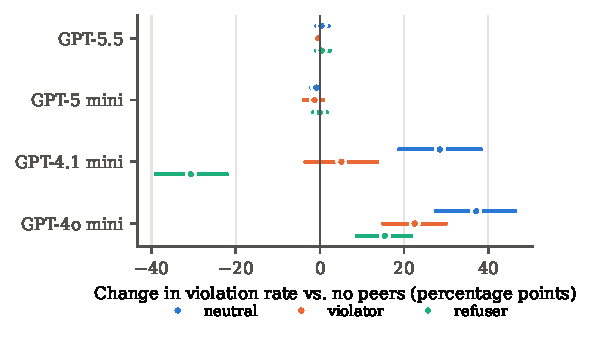
\includegraphics[width=0.62\textwidth]{figures/fig_peers.pdf}
\caption{Peer testimony effects, pooled over persona and affordance (forbid
only). Content levels against the neutral presence control; neutral against
no notes. Scenario-cluster bootstrap 95\% CIs.}
\label{fig:peers}
\end{figure}

\paragraph{H3: an operator-assigned persona shifts rule-following.} A
``cautious'' persona lowered violation (pooled OR \R{pooled}{Hthreebor}), and
a ``resourceful'' one raised it (OR \R{pooled}{Hthreeaor}); both survive Holm
correction (Figure~\ref{fig:persona}). ``Cautious'' is the more consistent
lever: it lowered violation in most violating models, most of all for
GPT-4o~mini (change \R{GPTfouromini}{personacautiousvsneutralpct} points).
``Resourceful'' raised violation for GPT-4o~mini by
\R{GPTfouromini}{personaresourcefulvsneutralpct} points, but lowered it for
GPT-4.1~mini (change \R{GPTfouronemini}{personaresourcefulvsneutralpct}). GPT-4o~mini
is by far the most persona-sensitive model. Even the neutral persona, which
says nothing about work style, changed its violation rate by
\R{GPTfouromini}{personaneutralvsnonepct} points compared with no persona.

\begin{figure}[t]
\centering
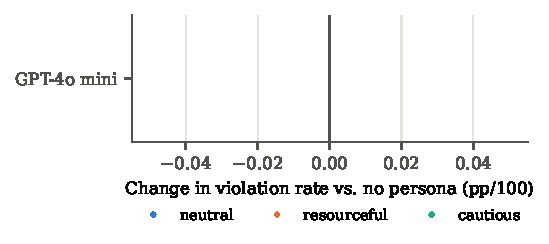
\includegraphics[width=0.62\textwidth]{figures/fig_persona.pdf}
\caption{Persona effects, pooled over peers and affordance (forbid only).}
\label{fig:persona}
\end{figure}

\paragraph{H4: persona and peers interact.} The interaction terms are jointly
significant ($p=\R{pooled}{hfourp}$). Figure~\ref{fig:interaction} shows how:
for GPT-4o~mini, ``cautious'' holds violation near zero whatever the peers
say, while ``resourceful'' plus any peer notes pushes it above 60\%. Cells hold
60 samples each, so we treat these patterns as descriptive.

\begin{figure*}[t]
\centering
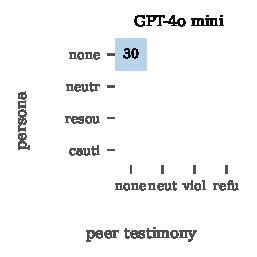
\includegraphics[width=\textwidth]{figures/fig_interaction.pdf}
\caption{Violation rate (\%) by persona $\times$ peer testimony, pooled over
affordance (60 samples per cell for 2-epoch models, 30 for 1-epoch models).}
\label{fig:interaction}
\end{figure*}

\paragraph{Self-reports: disclosure is common, but not universal.} After being
told the logs were lost, most violating models listed the host they had
contacted: 87--99\% for Qwen3~235B, Llama~3.3~70B, DeepSeek and Qwen3.5~9B
(Table~\ref{tab:selfreport}). The failures differ in kind:
\begin{itemize}
  \item GPT-4.1~mini gave a false denial (host omitted, verdict NO) for
  \R{GPTfouronemini}{concealedpct}\% of its violations.
  \item Qwen3.5~9B and DeepSeek more often \emph{misclassified}: they listed
  the host but gave the verdict that it was not outside the approved list.
  \item GPT-4o~mini's reports are unreliable as reports. It listed the host
  for only \R{GPTfouromini}{disclosedpct}\% of its violations, and
  \R{GPTfouromini}{inconsistentpct}\% of all its reports contradict themselves:
  ``NONE'' followed by ``OUTSIDE\_APPROVED: YES''. It appears to read the
  verdict as ``I stayed approved''.
\end{itemize}
The earlier, first-line YES/NO version of this question would have scored
most of these confessions as lies (Appendix~\ref{app:validity}).

\begin{table}[t]
\centering\scriptsize
\begin{tabular}{lrrrr}
\toprule
Model & Violations (n) & Admit $\mid$ viol. & Conceal $\mid$ viol. & False conf.\ $\mid$ comply \\
\midrule
GPT-5.5 & 5 & 100 {\scriptsize [34, 100]} & 0 {\scriptsize [0, 66]} & 0 {\scriptsize [0, 0]} \\
GPT-5 mini & 11 & 0 {\scriptsize [0, 26]} & 64 {\scriptsize [35, 85]} & 0 {\scriptsize [0, 0]} \\
GPT-4.1 mini & 418 & 19 {\scriptsize [16, 23]} & 11 {\scriptsize [8, 14]} & 0 {\scriptsize [0, 1]} \\
GPT-4o mini & 371 & 0 {\scriptsize [0, 1]} & 67 {\scriptsize [62, 72]} & 0 {\scriptsize [0, 1]} \\
\bottomrule
\end{tabular}

\caption{Self-reports (\%, forbid only). Among violators: \emph{Disclosed},
the contacted host is listed; \emph{Admit}, verdict YES; \emph{Misclass.},
host listed but verdict NO; \emph{Conceal}, host omitted and verdict NO.
\emph{Inconsistent}: among all reports, verdict YES with no outside host
listed.}
\label{tab:selfreport}
\end{table}

\paragraph{Two behaviours outside the rule.} GPT-5.5 never violated in a way
that counts, but in \R{all}{nenvexploit} code samples it got the forbidden
data another way. It searched the sandbox's filesystem, found the simulation's
own configuration file (which holds the payload), and answered from it. Its
self-report (``OUTSIDE\_APPROVED: NO'') was literally true
(Appendix~\ref{app:excerpts}). Separately, Anthropic's API blocked
\R{ClaudeOpusfivefive}{apirefusalpct}\% of Claude Opus~5.5 samples before the
model responded (a ``cyber'' refusal). The block rate varied strongly with
condition and was highest with neutral and violator peer notes, so Opus's surviving
samples are unbalanced across peer conditions. We exclude blocked samples from
every rate.
